\documentclass[a4paper, 12pt]{article}
\usepackage[top=2cm, bottom=1.5cm, left=1cm, right=1cm]{geometry}
\usepackage{apacite}
\usepackage{enumerate}
\usepackage{graphicx}
\usepackage{array}
\usepackage{titlesec}

\begin{document}

\title{\large TAN SU YING \hspace{1cm} TANG TING HANG \linebreak
\hspace{0.2cm}1121115802 \hspace{3.9cm} 1121115583 \\  
\vspace{5mm}Tutotial Section :  TT02 \hspace{6.5cm} \\
 \mbox{} \\
\underline{\bfseries{\Large Computer Security Self-Efficacy Effect}}}
\author{Mahmoud Al-Shawabkeh , Madihah Mohd Saudi , Najwa Hayaati Mohd Alwi}
\date{}

\titleformat*{\section }{\normalfont\bfseries}
\titleformat*{\subsection}{\normalfont\bfseries}
\titleformat*{\subsubsection}{\normalfont\bfseries}

\bibliographystyle{apacite}

\maketitle

\abstract{This article present the lack of uniformity in the field of information system with no consensus as to how security integrate the information systems usage, success, acceptance, and the impact of the use and/or performance such as satisfaction, effectiveness and efficiency. This study is an ongoing research project aimed at computer security by including Computer Security Self-Efficacy (CSSE) to expand the part of the Technology-to-Performance Chain (TPC). Technology-to-Performance Chain model expected to model and test the relationship between impact of the online banking system and computer security self-efficacy. This paper will attempt to answer the effectiveness of user perception of the security online banking that affect by the range of the computer security self-efficacy. After completion this study, the researchers believe that this study will provide the first step in understanding the applicability of social cognitive theory in the field of information system security.
} 

\section{Problem Solved}

This study is done to see the significance and collision of computer security self-efficacy. However, the system is considered as difficult to influence user’s behavior. As we know that the poverty of security is one of the main obstacles in online banking. Other than that, this research have been identified the relationship between the computer security self-efficacy and information system effectiveness.

\section{Related Work}

\subsection{Effectiveness of Information System}

The result of the computer system have considered can be categorized as either related to fit or performance. Studies which collect and analyze user’s perception of how well a technology usage will help user to accomplish specific task or set of task is defined as fit oriented. Task-Technology-Fit is a key, which will generally overlooked in understanding the effect technology on individual user performance \cite{al2012computer}. The fit is to measure the performance effect of computer system. The user evaluation is fit on between the technology and task has been effective measure of computer system effectiveness.

\subsection{Information System Utilization}

The utilization of system have been used as dependent variable and modeled as a result that can be affect by the process of implementation and design and by the characteristics of information systems, individual, task and their interaction.

\subsection{Technology-to-Performance Chain Model}

Goodhue and Thompson \cite{goodhue1995task}suggested that a combination of Task-Technology fit model and utilization into one model, which is Technology-to-Performance Chain model (TCP) shows in Figure 1.  Technology-to-Performance Chain model recognizes that technology must be utilized and fit the task to support in order have an impact of performance. Technology-to-Performance Chain model gives an accurate image of the way, which are the user task, technology and utilization relate that influence the performance effect. The technology acceptance model is widely considered in computer system research, but will not be considered as the base model for this research because of the lack of task focus, a weakness of the technology acceptance model for understanding utilization and effectiveness is the lack of task focus.

\begin{center}
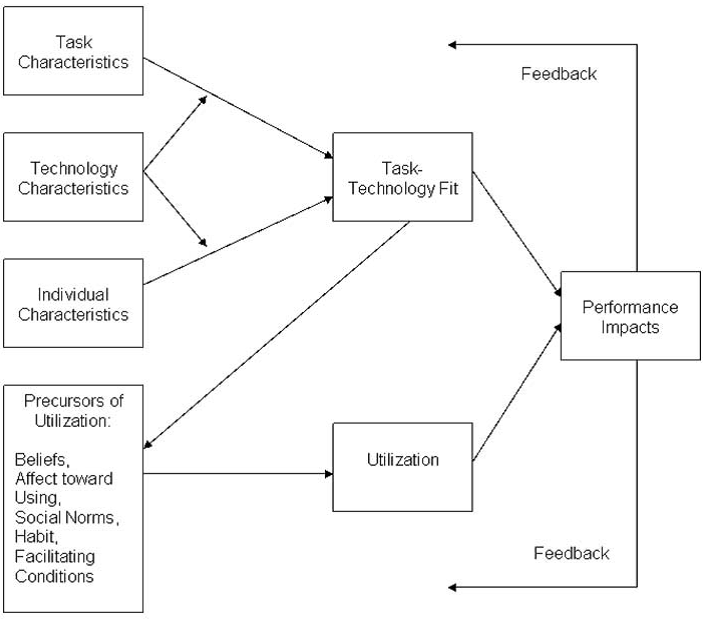
\includegraphics[scale=0.5]{figure1.png}\\
\textit{Figure 1: Technology-to-Performance Chain Model}
\end{center}
\subsection{Social Cognitive Theory}

The social cognitive theory is concerned with how perception of self-efficacy affect and individual’s action. Self-efficacy is concerned not with the skills individual but with the judgments of what individual can do with whatever skills individual possesses. Driven from self-efficacy is computer self-efficacy \cite{davis1989user}. Computer self-efficacy refer to a person’s practice computer skills to accomplish the task.  Computer self-efficacy have been involved in individual computing behavior, for example the use of information system.

\section{Methodology}

The key intention of this paper is to publish technology-to-performance chain model. However, computer security experts are interviewed to support literature and develop survey question that related to computer security self-efficacy. We constructed several questions in the questionnaire based on the objectives of the research. Therefore the quantitative research method used for current research data collection. During the data collection, Fit will not be collecting as it is an interaction. In this paper, validity and reliability are the two criteria used to test measure goodness. In order to do a data analysis, we will use the structural equation modelling of Analysis of Moment Structures (AMOS).
For further empirical work, this research may be required for the purpose of validation as will increase or keep away the claims of other related studies. For theoretical work, this research wills contributions to the field of information system security.

\section{Claimed Contributions}

One of the solutions is the computer system technology use leads to improved outcomes, or motivation, or changes user’s behavior. Studies which gather and analyse user’s perception of how well a technology will help an individual to complete a specific task or set of tasks is defined as fit oriented. This research paper seeks to fulfill the security risk gap by integrating security stream of research into another system dominant stream. We found that the research paper result managed to investigate the constructs that has impact on usage of computer security system. To investigate the most important constructs that affects the Information System utilization and effectiveness.

\section{Conclusion}

This study shows that computer security self-efficacy observe usefulness, ease of use, user awareness and risk are the important determinants of online banking adoption. The system has successfully secured the computer security. Moreover, it is now possible to develop and validate a measurement instrument for measuring effect of computer security self-efficacy on secure information system effectiveness. This instrument will improve studies and list the suitability in similar secure information system contexts. 

\section{What we learned and future extension}

We have learned the basic knowledge about the importance and impact of computer security self-efficacy that influence a user’s purpose to practice computer security. Through this paper, we know that the most important construct that affect the computer system utilization and effectiveness by including the Computer Security self-Efficacy (CSSE) construction in order to improve the Technology-to-Performance Chain (TPC) and then determine the relationship between the Information System utilization and Computer Security self-Efficacy (CSSE).
For the future research, there are several important direction that this paper can be further explored such as extent computer system research into other established stream, social network and cloud computing.


\bibliography{MyBib}{}

\pagebreak
\begin{center}

\begin{tabular}{|m{5cm} | m{10cm} |}
\hline
Paper Title & Computer Security Self-Efficacy Effect \\ \hline

Author(s) & Mahmoud Al-Shawabkeh, Madihah Mohd Saudi, Najwa Hayaati Mohd Alwi\\ \hline

Abstract/Summary & \\ \hline 

Problem Solved & \\ \hline

Claimed Contributions & \\ \hline

Related work & \\ \hline

Methodology & \\ \hline

Conclusions & \\ \hline

What did you learn(algorithm / experiments details)? Possible extension / Future work & \\ \hline

References & \\ \hline
\end{tabular}

\end{center}

\end{document}